\documentclass[11pt,a4j]{mybook2}
\usepackage[top=2.5cm, bottom=2.5cm, left=2cm, right=2cm]{geometry}
%\usepackage{showkeys}
%\documentclass[11pt,a4j]{jbook}
%\usepackage{graphicx,wrapfig}
\usepackage{graphicx,titlesec}
%\usepackage{tocloft} %目次の調整
%\setlength{\topmargin}{-1.5cm}
%\setlength{\textwidth}{16.5cm}
%\setlength{\textheight}{25.2cm}
\newlength{\minitwocolumn}
\setlength{\minitwocolumn}{0.5\textwidth}
\addtolength{\minitwocolumn}{-\columnsep}
%\addtolength{\baselineskip}{-0.1\baselineskip}
%
\def\Mmaru#1{{\ooalign{\hfil#1\/\hfil\crcr
\raise.167ex\hbox{\mathhexbox 20D}}}}
%
\newcommand{\fat}[1]{\mbox{\boldmath $#1$}}
\newcommand{\D}{\partial}
\newcommand{\w}{\omega}
\newcommand{\ga}{\alpha}
\newcommand{\gb}{\beta}
\newcommand{\gx}{\xi}
\newcommand{\gz}{\zeta}
\newcommand{\vhat}[1]{\hat{\fat{#1}}}
\newcommand{\spc}{\vspace{0.7\baselineskip}}
\newcommand{\halfspc}{\vspace{0.3\baselineskip}}
\bibliographystyle{unsrt}
\newcommand{\twofig}[2]
 {
   \begin{figure}
     \begin{minipage}[t]{\minitwocolumn}
         \begin{center}   #1
         \end{center}
     \end{minipage}
         \hspace{\columnsep}
     \begin{minipage}[t]{\minitwocolumn}
         \begin{center} #2
         \end{center}
     \end{minipage}
   \end{figure}
 }
%\titleformat{\chapter}[display]{\normalfont\normalsize}{\chaptertitlename \thechapter 章}{20pt}{\normalsize}
%{\normalsize}
%\vspace*{\baselineskip}
%\renewcommand{\cfttoctitlefont}{\hfill\normalsize\bfseries}
%\renewcommand{\cftaftertoctitle}{\hfill\null}
\renewcommand{\labelenumi}{(\arabic{enumi})}

\title{
\vspace{20mm}
圧縮成形された不飽和粘土の\\
電気化学インピーダンス特性に関する研究
\\
\vspace{5mm}
Study on Chemical Impedance Characteristics 
of Unsaturated Compacted Clay
\vspace{60mm}
}
%\date{\today}
\date{2021年2月9日}
\author{
	\vspace{40mm}
岡山大学環境理工学部\\
環境デザイン工学科 10429223\\
	佐々木 絢悟
}

%\makeatletter
%\def\@evenfoot{\hfil -\thepage- \hfil}
%\makeatother
%\makeatletter
%\def\@oddfoot{\hfil -\thepage- \hfil}
%\makeatother
%\makeatletter
%\def\@oddeven{}
%\makeatother

\begin{document}
\maketitle
%-------------------------
\begin{center}
\begin{minipage}{15cm}
\begin{center}
	{\bf 要旨}
\end{center}
本研究は圧縮成形された不飽和粘土の電気化学インピーダンス特性を実験によって調べたものである.
実験には,Na型モンモリロナイトと純水を混合して圧縮し,ペレット状に成形した供試体を用いた.
供試体は5つの異なる含水比で作成し,各々,圧縮途上で所定の厚みにおいてインピーダンスを計測する
ことで水分量と乾燥密度の影響を調べた. 実験の結果,不飽和粘土のインピーダンススペクトルは
Cole-Coleプロットで近似できることが分かった.
Cole-Coleプロットの等価回路には,互いに並列接続された抵抗とCPE(constant phase element)が
含まれ,CPEは2つの素子定数を持つ.そこで,これら2つの定数をカーブフィッテイングを行って
求めたところ,いずれの定数も含水比と乾燥密度に関して明確な相関を示すことが明らかとなった.
特に,CPE定数の一つである指数$p$は特異な挙動を示し,含水比が$20\%$を超えるときには乾燥密度
と正の相関を持つが,それ以下では負の相関を示すことが分かった.このことは,
指数$p$は不飽和粘土の間隙や間隙水の配置に関する微視的な構造変化を捉える指標に
なりうるという意味で有用な知見と言える.
	\vspace{15mm}
\begin{center}
	{\bf ABSTRACT}
\end{center}
This study investigates the characteristics of the electrochemical impedance of compacted clay by experiment.
For the experiment, clay pellets of five different water contents were made by compacting moistured Na-montmorillonite.
During the compaction, the impedance was measured when the pellet is compressed to the predetermined heights. 
In this way, the impedance at several different bluk densities were obtained.
Over the range of water conent and bulk density considered,  the impedance spectra are found to be 
approximated by a Cole-Cole type plot. The equivalent circuit for the Cole-Cole plot includes the parallell-connected 
resisntance and CPE(constant phase element). The two CPE parameters were hence estimated by fitting the theoretical 
to the measuremets impedance. The estimated constants showed clear correlation with both the dry bulk density 
and the water content. Among the two constants, the exponent $p$ of the CPE was found to behave in a more peculiar way. 
Specifically, $p$ scales negatively with the increase in the dry density when the water content is greater than 20\%. 
For lower water content, on the contrary, it scales positively against the dry density. 
This is an important finding that suggests the CPE expoent can be an indicator of a microstructural change 
related to the pore and pore water structure of the compacted clay.
\end{minipage}
\end{center}
%-------------------------
\tableofcontents
\frontmatter
\mainmatter
%%%%%%%%%%%%%%%%%%%%%%%%%%%%%%%%%%%%%%%%%%%%%%%%%%%%%%%%%%%%%%%%
%\chapter{はじめに}
	%\chapter{はじめに}
\section{研究の背景}
%
%	鋼構造,非破壊検査,超音波探傷,きずの検出と評価
%
我が国には,高度成長期に建設され老朽化の進む橋梁が数多く存在し,そこには鋼橋梁も多数含まれる. 
鋼橋梁の劣化は主として腐食と疲労で進行する.
疲労は,繰り返し載荷によってき裂が発生,進展する劣化現象で,応力集中や断面欠損で橋梁の耐荷力を低下させる.疲労き裂は溶接継手部で発生することから,疲労損傷の予防や補修のためには,溶接部におけるき裂の発生や進展挙動について理解することが必要となる\cite{Miki}.
その際,き裂の起点となるブローホールや融合不良といった溶接欠陥の有無や,すでにき裂が生じている場合はき裂自身の位置や大きさを知ることが重要となる.
き裂に関して言えば,部材表面に開口した表面き裂として存在する場合もあるが,き裂進展部に当たる先端は部材内にあり,目視検査だけで大きさや向きを知ることはできない.
さらに,き裂の開口部が,例えば閉断面リブ内側にあるような場合には,部材表面であってもき裂位置を直接観察することはできない.
以上のことから,溶接継手部の探傷には固体内部の状態を観察することのできる各種非破壊検査法が用いられる.
代表的な非破壊検査法には,磁粉探傷法,X線透過試験,超音波探傷法,渦電流法,サーモグラフィー
による欠陥検出法などがある.磁粉探傷法は目視検査の一種で,内部き裂を検出することはできない.
また,X線透過試験は厚板には適用できず,放射線遮蔽の問題もあり現場探傷には不向きである.
一方,渦電流法やサーモグラフィーは表面付近のき裂検出に適するものの,内部き裂の検出やサイズの評価は得意でない.これに対して超音波探傷試験では,固体内部を伝播する弾性波の一種である超音波エコーを観察することでき裂の検出や評価を行う.超音波探傷のための装置は原理的には単純かつ比較的安価に構築することができ,
安全上の問題もない.また,検査に用いる超音波のモードや周波数を適切に選べば,内部欠陥の検出や評価が可能で,これらの点で現場探傷のための非破壊検査法として他の手法には無い利点がある\\

%
%	UTの原理と課題(複数経路,形状エコー)
%
超音波探傷試験では,圧電素子やレーザを使って超音波を試験体に励起する.
超音波は,き裂や介在物など,密度や剛性が変化する欠陥(きず)部位で反射,散乱されて超音波エコーが発生する.このことから,きずからの超音波エコーを物体表面で観察することにより,物体内部に不均一部や界面が存在することを検知できる.
さらに,超音波の伝播速度が既知であれば,入射波の送信時刻とエコー到達時刻から伝播時間が求まり,伝播時間からきずまでの距離を知ることができる.このような作業を多数の点で行い距離情報を集めれば,超音波エコー波形から,きずの正確な位置が得られる.また,得られた波形をトモグラフィー処理するなどして可視化すれば,欠陥の像(イメージ)として分かりやすく表示することもできる.このように超音波探傷法は,エコーの伝播時間を距離に換算して位置特定を行うという原理的には単純なものである\cite{US}.一方で,超音波探傷法を溶接継手の検査に適用する場合,伝播時間や距離の決定は必ずしも簡単ではない.
まず,超音波エコーの発生源は検出すべきき裂だけに限られない.
例えば,溶接止端部や部材端の角部など,急な形状変化がある箇所では回折波が生じ,計測波形に複数のエコーが場合いよっては同時刻に現れる.これら複数のエコーのうち,きずからのエコーは通常,微弱で,不要なエコーに隠され探傷波形上、簡単には特定できない.さらに,固体内部の超音波の伝播挙動は複雑で,縦波や横波に加えて,
表面波や界面波も含む複数のモードが発生する\cite{JDA}.これらの波動モードは反射や散乱時に互いに変換が起きる(モード変換)ため,一つのきずを検出する場合も,可能なエコー伝播経路が複数存在する.また,それら複数の経路を経たエコーのいずれが実際に観測されるかを判定する簡単な基準も存在しない.\\

%
%	エコー振幅や伝播経路の解析(波線理論と数値波動解析)
%
以上のように,超音波による溶接継手の探傷では,不要なエコー(形状エコー)ときずエコーの分別と,エコー伝播経路の特定が課題となる.可能なエコー伝播経路は,概ね波線理論(ray theory)によって調べることができる\cite{JDA}.波線理論は波動伝播に関する近似理論で,高周波数の波は均質材中を波線(ray)と呼ばれる直線に沿って伝播すると考える.また,物体表面ではスネルの法則によって反射や屈折,モード変換を起こすと考える.波線理論は伝播時間や経路に関する限り,フェルマーの原理やホイヘンスの原理と同じ結果を与える.一方,波線に沿った振幅変化を計算するのは困難が多く,特に,回折波や表面波が発生する状況では限られたケースでしか波線理論解析が有効でない.このことは,可能な経路とその伝播時間の見積りは波線理論である程度可能だが,振幅値を予想してエコー強度を予想し,特定の経路を経たエコーが観測されるかどうかを波線理論的な検討から判断するのは難しいことを意味する.
これに対して,有限要素法や差分法による数値波動解析では,縦波や横波,表面波等の非実体波を区別することなく,任意の物性値や形状で波動場の計算が可能である.
固体中の超音波は弾性波の一種で振幅も小さく,微小変形理論を適用し線形弾性体として扱うことができる.
従って,線形弾性固体の運動方程式を与えられた初期値,境界値の元で計算することで,任意の時間と位置における超音波の振幅や位相を計算することができる.こういった波動解析は,計算負荷は依然として大きいものの,これまでの数値解析技術と計算機環境の整備により,今日では実施自体はそれほど難しいものではない.しかしながら,数値波動解析の結果では,種々のモードが混在した複雑な波動場が得られるために,数値解析結果を解釈することも結局は簡単でない.特に,数値計算で予想されたエコーがどのような経路を辿ったものかについては,数値解析結果に明示的に示される訳でなく,超音波探傷結果の理解を自動的に深めてくれる状況には至っていない.\\

%
%	溶接継手部の超音波探傷(形状エコ-,送受信位置,モードの問題)
%
きずエコ-が,周辺で発生する形状エコーで隠され検出困難となる状況は,ごく簡単な継ぎ手形状でも発生する.きずの無い板であれば、内部にどのうような波動場が生じるかは理論的に詳しく調べられ,薄板ではLamb波と呼ばれるガイド波が生じることが知られている.突き合わせ溶接継手は,溶接ビードの部分を除けば、概ね板材とみなすことができるため,この状況に当てはまる.一方,基本的な継ぎ手形式であるT継手では,きずが存在しない場合も波動場の理論解は得られない.そのため,波動場解析は数値解析に依らざるを得ない.
T継手では,継手部分の角部で回折波が生じる.さらに,き裂が存在する場合には,角部からの回折波がき裂でも散乱され,複雑な多重散乱場を形成する.また,実際の継手部には溶接ビードが存在するため,ビード内部や表面での反射は,継手周辺の平板部分と大きくことなる波動伝播形態を示す.
これらのことが相俟って,継手形状としては単純なT継手でも,超音波伝播挙動は複雑になり得る.
従って,継手周辺での波動伝播挙動を正確に理解し,観測可能なエコーの発生メカニズムと伝搬挙動を把握することは超音波探傷試験の適切な実施の上で重要である.
\section{研究の目的}
以上を踏まえ本研究では,T溶接継手におけるきずエコーの発生および伝播挙動を理解することを目的とした数値シミュレーションを行う.具体的には,T継手角部から発生してフランジ側へ伸びるき裂を対象として,き裂に到達する入射波と,それによって励起されるする散乱波の挙動を調べる.超音波の送受信はフランジの一方の面で,き裂に対して片側からのみ可能と仮定する、制約の厳しい計測条件を想定したシミュレーションを行う.
数値シミュレーションにはFDTD法(時間領域有限差分法finit difference time domain method)\cite{FDTD1},\cite{FDTD2}を用い,模擬探傷波形データを合成する.この波形中に含まれる主要なき裂エコーが,いつどのようにして発生,伝搬したかをFDTD法によって部材内部の波動場観察から明らかにする.
これら一連の計算結果の示す知見を,T継手の超音波探傷試験の観点から整理,考察する.
\section{本論文の構成}
本論文の構成を以下に述べる.
本章で述べた研究背景と目的に続き,第二章では超音波探傷シミュレーションの問題設定と数値波動解析法について示す.ここでは,想定する継手形状や探傷条件,波動場の支配方程式と数値解析法について述べる.
第三章では,簡単な形状のモデルで行ったシミュレーションの結果を示す.シミュレーションは,
基礎モデルとして平板と簡易なT継手モデルで行い,各々,どのような入射波と散乱波が発生するかを見る.
第4章では,より現実的なモデルとして,T溶接継手の余盛形状をモデルに取り込んだ詳細なシミュレーションを行う.これは,近年,疲労損傷が問題となっている,鋼床版Uリブのすみ肉溶接部に発生するき裂の探傷を模擬したものである\cite{Urib1},\cite{Urib2},\cite{Urib3}.溶接部の複雑な形状がエコー形成に与える影響を調べ,どのような送受条件で有用なきずエコーが観測可能であるかをこのシミュレーションを通じて明らかにする.
最終,第5章では本研究で得られた知見をまとめ,結論と今後の課題を示す.なお,本研究では計算効率の制約のため全ての数値シミュレーションを2次元問題として行う.


%\chapter{スメクタイト族粘土の結晶構造,分類,特徴}
	%\chapter{超音波擔傷試験の数値シミュレーション法}
\section{問題設定}
図\ref{fig:}に、本研究で想定するT字継手における超音探傷試験の状況設定を示す。
継手は、水平部材に対して直角に近い角度で板材が溶接されているとし、
以下、便宜上、水平部材をウェブ、鉛直向きの板材をフランジと呼ぶ。
溶接部の詳細はこの図には示していないが、片側(右側)からの隅肉溶接が行われているとし、
継手右側を外側、左側を内側と称する。
なお、次章で示す数値シミュレーション結果では、比較のために、溶接部の余盛りを無視し、
ウェブとフランジが溶接金属が追加されることなくそのまま結合されたモデルや、
厚みが一定の平板に対する結果も示す。
き裂は、継手内側の角部から発生してウェブ側へ鉛直に近い方向へ伸びるものを考える。
現実には、継手に生じる応力場によってき裂の進展方向は変化するため、起点が同じでも
溶接金属内やウェブ側にき裂が伸びるケースもある。それらは、ウェブ側からの探傷が
必要で、超音波の送受信や伝播状況が図のものと大きくことなるため、別途、考察の
対象とする必要があるため、本研究では扱わない。
超音波の送受信は、継手外側のフランジ上側の面でのみ実施可能とする。
従って、送信、受信方向はき裂に対して強く制約され、検査に利用できる超音波エコーは
き裂からの後方散乱波だけとなる。もし、
送受信をき裂を挟むように、継手左右両側から行うことができるならば、
よく知られたTOFD法(time-of-flight diffraction)が利用できる。
ここでは、TOFDが適用できない状況がより困難で、詳細な検討を要する問題であるため、
片側からの探傷を扱う.
超音波の送信は、鋼橋の超音波探傷で通常用いられる圧電探触子で、フランジ上面から
行う。ただし、数値シミュレーションでは、圧電素子を直接モデル化することは避け、
既知の鉛直な表面力分布で与える。この方法では、表面力の時間変化に位相差が内場合、
探触子からの垂直入射を、直線的な位相差をつけることで斜角入射を模擬することができる。
受信は無指向性の点レシーバにより、継手外側の任意の範囲で行うことができるとする。
これは、波長に対して十分に小さいアレイ探触子での受信を想定したものである。
実際の探傷は、必ずしもアレイセンサーを用いる場合ばかりでは無いが、
アレイセンサーで受信した波形群を適切な遅延時間を設けて重ね合わせることで、
斜角探触子による受信も模擬できるため、この意味で、今回の設定は、一般のセンサー
による受信波形を模擬できる点でより包括的なものと言える。
\section{波動伝播問題の定式化}
鋼橋の超音波探傷試験に用いる超音波の周波数帯は、およそ2MHzから5MHzで、
その振幅は数十nm程度と非常に小さい。そのため、超音波伝搬は微小変形問題で、
媒体は線形弾性体とみなした解析を行うことができる。
このとき、弾性波動問題の支配方程式は、応力$\sigma_{ij}$, 速度$v_i$,
質量密度$\rho$を用いて
\begin{equation}
	\sigma_{ji,j}+f_i=\rho \dot{v}_i,
	\label{eqn:}
\end{equation}
ただし,$(,)$は空間の$\dot{()}$は時間に関する微分
\begin{equation}
	(\cdot)_{,i}=\frac{\partial (\cdot)}{\partial x_i}, \ \ 
	\dot{(\cdot)}=\frac{\partial (\cdot)}{\partial x_i}, \ \ 
	\label{eqn:}
\end{equation}
をそれぞれ表す.
2次元問題を考えるため、インデックス$i,j$は1または2で、総和規約を用いている.
速度$v_i$は変位$u_i$の時間微分であり、ひずみテンソル$\varepsilon_{ij}$は、
変位を使って
\begin{equation}
	\varepsilon_{ij}=\frac{1}{2}(u_{i,j}+u_{j,i})
	\label{eqn:}
\end{equation}
で、応力テンソルは弾性係数テンソル$C_{ijkl}$として
を用いて次のように表される。
\begin{equation}
	\varepsilon_{ij}=C_{ijkl}\varepsilon_{kl}
	\label{eqn:}
\end{equation}
ただし、ここでは媒体は等方性体とみなし、
\begin{equation}
	C_{ijkl}=\lambda \delta_{ij}\delta_{kl} +\mu \delta_{ik}\delta_{jl}
	\label{eqn:}
\end{equation}
とする。ここに、$\lambda, \mu$はラメ定数を表す。ラメ定数と密度より、
縦波と横波の位相速度は、順に
\begin{equation}
	c_{P}=\sqrt{\frac{\lambda + 2\mu}{\rho}}
	, \ \ 
	c_{S}=\sqrt{\frac{\mu}{\rho}}
	\label{eqn:}
\end{equation}
と与えられる.工学でしばしば用いられるヤング率$E$,ポアソン比$\nu$,せん断剛性$G$を
用いれば、ラメ定数は
\begin{equation}
	G=\mu, 
	\label{eqn:}
\end{equation}
$\mu$はせん断合成に一致している。
以上の式を与えられた初期条件、境界条件の元で解くことで、超音波の伝播シミュレーションを行うことができる。
\section{数値解析法(FDTD法)}
前節で示した方程式に離散化に,FDTD(Finite Difference Time-Domain)法を用いる.
時間ステップ長を$\Delta t$, スタガード格子の$x_i$軸方向の間隔を
$\Delta x_i,(i=1,2)$とし,その間隔は一定とする.この間隔で時空間内に配置された差分格子における関数$f(\fat{x},t)$の値を$f^k_{i,j}$と書くことにする.ただし,$k$は時間ステップを,$i,\, j$は$x_1$および$x_2$方向の格子位置を表す番号を意味する.このとき,中央差分で時間微分を近似すれば,
\begin{equation}
	\dot{f}^{k+\frac{1}{2}} \approx \frac{ (f)^{k+1}-(f)^k}{\Delta t}
	\label{eqn:dfdt}
\end{equation}
となり,後に示すように,整数時間ステップ$k$で$f^k$を,半整数時間ステップ$t^{k+\frac{1}{2}}$において$\dot f$を,初期値$f^0, \dot f^{\frac{1}{2}}$から交互に求める蛙飛び差分法による差分方程式が得られる.一方,空間微分$\nabla f$は
\begin{eqnarray}
	\left( \frac{\partial f}{\partial x_1}\right)
	_{i+\frac{1}{2}, \, j+\frac{1}{2}}
	& \approx &
		\frac{\left(f\right)_{i+1,j+\frac{1}{2}} -\left(f\right)_{i,\, j+\frac{1}{2}}}
		{\Delta x_1}
	\label{eqn:dfdx1}
	\\
	\left( \frac{\partial f}{\partial x_2}\right)
	_{i+\frac{1}{2}, \, j+\frac{1}{2}}
	& \approx &
	\frac{\left(f\right)_{i+\frac{1}{2},j+1} -\left(f\right)_{i+\frac{1}{2},\, j}}{\Delta x_2}
	\label{eqn:dfdx2}
\end{eqnarray}
と近似する.このような差分化を行うためには,関数$f$とその勾配$\nabla f$の計算格子がスタガード格子を形成するように配置しておけばよい.
%%%%%%%% FIGURE 2 %%%%%%%%%
%	FD GRID
\begin{figure}
     \begin{center}
     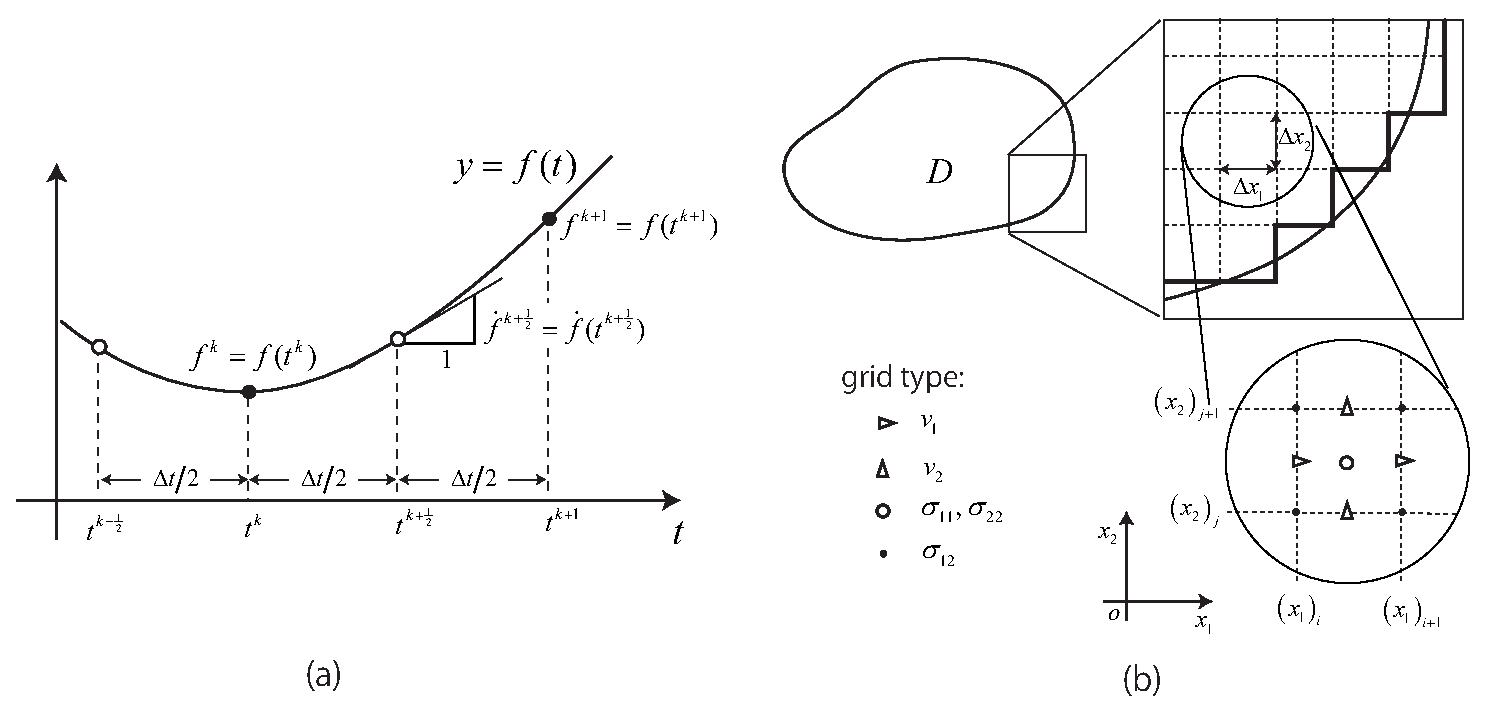
\includegraphics[width=1.0\linewidth]{Figs/FDgrid.eps}
     \end{center}
     \caption{ (a) Finite difference grid arrangement for leap-frog time stepping scheme.
	 (b) The staggered grid system for the central difference approximation 
		of spatial derivatives appearing in the governing elastoynamic 
		equations. A close-up of the unit FD-cell is also shown.
	}
     \label{fig:FDgrids}
\end{figure}
%%%%%%%%%%%%%%%%%%%%%%%%%%%
スタガード格子は図\ref{fig:FDgrids}に示したような,直応力の計算格子を中心にした
$\Delta x_1 \times \Delta x_2$の矩形領域の頂点にせん断応力の,辺上に速度の計算格子を配置したセルを基本単位とする格子配置をとる.これらの格子点における関数値を用いて, 動弾性問題の支配方程式を差分近似すれば,以下のような結果が得られる.
\begin{equation}
	\rho \frac{(v_1)_{i,j+\frac{1}{2}}^{k+1}-(v_1)^k_{i,j+\frac{1}{2}}}{\Delta t}
	=
	\frac{ 
		(\sigma_{11})^{k+\frac{1}{2}}_{i+\frac{1}{2},j+\frac{1}{2}}
		-(\sigma_{11})^{k+\frac{1}{2}}_{i-\frac{1}{2},j+\frac{1}{2}} 
	}
	{\Delta x_1}
	+
	\frac{(\sigma_{12})^{k+\frac{1}{2}}_{i,j+1}-(\sigma_{12})^{k+\frac{1}{2}}_{i,j}}{\Delta x_2}
	\label{eqn:fdtd_v1}
\end{equation}
\begin{equation}
	\rho \frac{(v_2)_{i+\frac{1}{2},j}^{k+1}-(v_2)^k_{i+\frac{1}{2},j}}{\Delta t}
	=
	\frac{(\sigma_{12})^{k+\frac{1}{2}}_{i+1,j}-(\sigma_{12})^{k+\frac{1}{2}}_{i,j}}{\Delta x_1}
	+
	\frac{ 
		(\sigma_{22})^{k+\frac{1}{2}}_{i+\frac{1}{2},j+\frac{1}{2}}
		-(\sigma_{22})^{k+\frac{1}{2}}_{i+\frac{1}{2},j-\frac{1}{2}} 
	}
	{\Delta x_2}
	\label{eqn:fdtd_v2}
\end{equation}
\begin{equation}
	\frac{
		 (\sigma_{11})^{k+\frac{1}{2}}_{i+\frac{1}{2},j+\frac{1}{2}}
		-
		 (\sigma_{11})^{k-\frac{1}{2}}_{i+\frac{1}{2},j+\frac{1}{2}}
	}
	{\Delta t}
	=
	\left( \lambda+2\mu \right)
	\frac{
		(v_1)^{k}_{i+1,j+\frac{1}{2}} - (v_1)^{k}_{i,j+\frac{1}{2}} 
	}
	{\Delta x_1}
	+
	\lambda
	\frac{
		(v_2)^{k}_{i+\frac{1}{2}, j+1} - (v_2)^{k}_{i+\frac{1}{2},j} 
	}
	{\Delta x_2}
	\label{eqn:fdtd_s11}
\end{equation}
\begin{equation}
	\frac{
		 (\sigma_{22})^{k+\frac{1}{2}}_{i+\frac{1}{2},j+\frac{1}{2}}
		-
		 (\sigma_{22})^{k-\frac{1}{2}}_{i+\frac{1}{2},j+\frac{1}{2}}
	}
	{\Delta t}
	=
	\lambda
	\frac{
		(v_1)^{k}_{i+1,j+\frac{1}{2}} - (v_1)^{k}_{i,j+\frac{1}{2}} 
	}
	{\Delta x_1}
	+
	\left( \lambda+2\mu \right)
	\frac{
		(v_2)^{k}_{i+\frac{1}{2}, j+1} - (v_2)^{k}_{i+\frac{1}{2},j} 
	}
	{\Delta x_2}
	\label{eqn:fdtd_s22}
\end{equation}
\begin{equation}
	\frac{
		 (\sigma_{12})^{k+\frac{1}{2}}_{i,j}
		-
		 (\sigma_{12})^{k-\frac{1}{2}}_{i,j}
	}
	{\Delta t}
	=
	\mu \left(
		\frac{
			(v_2)^{k}_{i+\frac{1}{2},j}
			-
			(v_2)^{k}_{i-\frac{1}{2},j}
		}
		{\Delta x_1}
		+
		\frac{
			(v_1)^{k}_{i,j+\frac{1}{2}}
			-
			(v_1)^{k}_{i,j-\frac{1}{2}}
		}
		{\Delta x_2}
	\right)	
	\label{eqn:fdtd_s12}
\end{equation}
以上の式のうち,式(\ref{eqn:fdtd_v1})から(\ref{eqn:fdtd_v2})を,$(v_1)^{k+1}_{i,j+\frac{1}{2}}$や$(v_2)^{k+1}_{i+\frac{1}{2},j}$について解けば, 速度と応力を交替に求める蛙飛び差分スキームによる差分公式が得られる.なお,以上の結果は領域内部にある計算格子において適用可能なものであるため,境界上のグリッドについては,指定された境界条件を反映した差分方程式を用いる必要がある.ここでは,トラクションが与えられた境界における境界条件の与え方について述べる.いま,計算領域を差分セルの集合で近似することを考えると,境界上に配置される可能性のある計算格子は$v_1, v_2$および$\sigma_{12}$である.このうち$\sigma_{12}$については,与えらえた境界値をそのまま代入すればよい.一方,速度$v_1, v_2$については,単位セルサイズが半分になったものと考え,運動方程式を有限体積法の考え方に従って離散化すれば,次のような差分方程式が得られる.
\begin{equation}
	\rho \frac{(v_1)_{i,j+\frac{1}{2}}^{k+1}-(v_1)^k_{i,j+\frac{1}{2}}}{\Delta t}
	=
	\alpha
	\frac{ 
		(\bar\sigma_{11})^{k+\frac{1}{2}}_{i,j+\frac{1}{2}}
		-(\sigma_{11})^{k+\frac{1}{2}}_{i-\frac{\alpha}{2},j+\frac{1}{2}} 
	}
	{\Delta x_1/2}
	+
	\frac{(\bar \sigma_{12})^{k+\frac{1}{2}}_{i,j+1}-(\bar \sigma_{12})^{k+\frac{1}{2}}_{i,j}}{\Delta x_2}
	\label{eqn:fdtd_v1_bnd}
\end{equation}
\begin{equation}
	\rho \frac{(v_2)_{i+\frac{1}{2},j}^{k+1}-(v_2)^k_{i+\frac{1}{2},j}}{\Delta t}
	=
	\frac{(\bar\sigma_{12})^{k+\frac{1}{2}}_{i+1,j}-(\bar\sigma_{12})^{k+\frac{1}{2}}_{i,j}}{\Delta x_1}
	+
	\beta
	\frac{ 
		(\bar \sigma_{22})^{k+\frac{1}{2}}_{i+\frac{1}{2},j}
		-(\sigma_{22})^{k+\frac{1}{2}}_{i+\frac{1}{2},j-\frac{\beta}{2}} 
	}
	{\Delta x_2/2}
	\label{eqn:fdtd_v2_bnd}
\end{equation}
ただし,$\bar{(\cdot)}$は既知の境界値であることを意味し,式(\ref{eqn:fdtd_v1_bnd})と(\ref{eqn:fdtd_v2_bnd})に含まれるパラメータ$\alpha$および$\beta$は,
 \begin{equation}
	\alpha=(n_1)_{i,j+\frac{1}{2}}, \ \ \beta=(n_2)_{i+\frac{1}{2},\, j},
	\label{eqn:def_ab}
\end{equation}
で,外向き法線ベクトル$\fat{n}=(n_1,\, n_2)$の方向により1または-1をとる.以上を用いて,弾性波の2次元伝播散乱解析を行った結果を次節に示す.
%%%%%%%%%%

%\chapter{電気化学インピーダンス法の基礎}
%	\chapter{電気化学インピーダンス法の基礎}
\section{インピーダンス}
電気化学インピーダンス法では試料に交流電圧を印加し,その応答として生じる電流を計測する.
電流$I$と電圧$V$の関係が線形システムとみなせるならば,両者の関係は
\begin{equation}
	V(\omega)= Z(\omega) I(\omega), \ \ (\omega=2\pi f)
	\label{eqn:I2V}
\end{equation}
と表すことができる.ここに,$\omega$と$f$はそれぞれ交流電圧の角周波数[rad/s]と周波数[Hz]を表す.
なお,時間因子$e^{i\omega t}$は両辺に共通のため省略する.
このとき,電流と電圧の比である$Z$はインピーダンスと呼ばれる.
$Z$も周波数の関数であることから,$Z$はインピーダンススペクトルとも呼ばれる.
インピーダンス$Z(\omega)$は一般に複素数で,虚数単位を$i$として
\begin{equation}
	Z(\omega)=Z'(\omega)+iZ''(\omega)
	\label{eqn:Z_cmplx}
\end{equation}
と実部,虚部を書く.$Z'$はレジスタンス,$Z''$はリアクタンスと呼ばれる.
インピーダンスは指数関数を用いて
\begin{equation}
	Z(\omega)=\left| Z \right|(\omega)e ^{i\phi(\omega)}
	\label{eqn:}
\end{equation}
と表すこともできる.ここで$\phi$は複素数$Z$の偏角を表し,
$\phi$は電流と電圧の間の位相遅れを意味する.
%
\section{インピーダンススペクトルの表示方法}
インピーダンススペクトルの表示は目的に応じて二種類の方法が用いられる.
1つめの方法では横軸に周波数を,縦軸にインピーダンスの大きさ$|Z|$をとり
両対数グラフとして表示するものである.同時に,横軸を対数軸として周波数に,
縦軸を$Z$の偏角$\phi$としたグラフを合わせて見ることで,
インピーダンススペクトルの完全な情報を示すことができる.
これらの2つのグラフによる表示をBode(ボード)線図と呼ぶ.
もう一つの方法は,横軸にレジスタンス$R'$を,縦軸をリアクタンスの符号を反転
させた$-R''$とした複素平面にインピーダンス$Z$をプロットするものである.
各周波数におけるインピーダンスをこのような複素平面上にプロットすれば,
インピーダンススペクトルが複素平面上の曲線として表される.このような
インピーダンススペクトルの表示はNyquist(ナイキスト)線図と呼ばれる.
Nyquist線図はインピーダンススペクトの特徴をしばしば直感的にわかり易く示してくれる.
ただし,周波数に対する依存性はNyquist線図上で明示的に示されない.
そのため,周波数との関係を同時に見る必要がある場合には,Bode線図も併用する
ことになる.
%
\section{等価回路}
実験やシミュレーションで得られたインピーダンススペクトルを再現できる
簡単な電気回路を,対象とする試料やモデルの等価回路(equivalent circuit)と呼ぶ.
等価回路を構成する最も基本的な回路素子には抵抗($R$),コンデンサ$(C)$,
インダクタンス$(L)$の3つがある.
回路が理想的な抵抗だけからなる場合,電流と電圧の関係はオームの法則により
\begin{equation}
	V=RI
	\label{eqn:Ohom}
\end{equation}
で与えられる.この場合,インピーダンスは$Z=R$で周波数に依らず,
ボード線図とナイキスト線図はそれぞれ図\ref{fig:fig3_1}に示したようになる.
一方,コンデンサ-だけからなる回路では,電圧と帯電量$Q$の関係:
\begin{equation}
	V=\frac{Q}{C}
	\label{eqn:Q_CV}
\end{equation}
より,
\begin{equation}
	\frac{dV}{dt}=i\omega V =\frac{1}{C}\frac{dQ}{dt}=\frac{I}{C}
	\label{eqn:}
\end{equation}
だから,インピーダンスは
\begin{equation}
	Z=\frac{1}{i\omega C}
	\label{eqn:Zc}
\end{equation}
で与えられリアクタンス成分だけを持つ.
図\ref{fig:fig3_2}はこの結果を示したナイキスト線図とボード線図である.
また,本研究で用いることは無いが,インダクタンスのみの回路については
電流と起電力の関係:
\begin{equation}
	V=-L\frac{dI}{dt}=-i\omega LI 
	\label{eqn:}
\end{equation}
より
\begin{equation}
	Z=i\omega L
	\label{eqn:}
\end{equation}
で,コンデンサと同様リアクタンス成分だけになる.
この場合のインピーダンススペクトルは図\ref{fig:fig3_3}の通りである.
なお,以上の図\ref{fig:fig3_1}-図\ref{fig:fig3_3}においてナイキスト線図
に示した青の矢印は,低周波から高周波側に進む方向を示している.
%--------------------
\begin{figure}[h]
	\begin{center}
	\includegraphics[width=0.9\linewidth]{Figs/fig3_1.eps} 
	\end{center}
	\caption{
		抵抗素子のボード線図(a),(b)とナイキスト線図(c).
	} 
	\label{fig:fig3_1}
\end{figure}
%--------------------
%--------------------
\begin{figure}[h]
	\begin{center}
	\includegraphics[width=0.9\linewidth]{Figs/fig3_2.eps} 
	\end{center}
	\caption{
		コンデンサ素子のボード線図(a),(b)とナイキスト線図(c).
	} 
	\label{fig:fig3_2}
\end{figure}
%--------------------
%--------------------
\begin{figure}[h]
	\begin{center}
	\includegraphics[width=0.9\linewidth]{Figs/fig3_3.eps} 
	\end{center}
	\caption{
		インダクター素子のボード線図(a),(b)とナイキスト線図(c).
	} 
	\label{fig:fig3_3}
\end{figure}
%--------------------
以上に述べた基本的な回路素子を組み合わせることで,より多様なインピーダンススペクトルを表現することができる.
そのような例として以下では,本研究に関連の深い5つの回路を取り上げ,そのインピーダンススペクトルを示す.
\section{合成インピーダンス}
\subsection{RC並列回路}
抵抗$R$とコンデンサ$C$を並列に接続したRC並列回路の合成インピーダンスは
\begin{equation}
	\frac{1}{Z}=\frac{1}{R} + i\omega C \ \ 
	\Rightarrow \ \ Z =\frac{R}{1+i\omega RC}
	\label{eqn:RC_para}
\end{equation}
で与えられる.従ってレジスタンス$Z'$とリアクタンス$Z''$は,それぞれ
\begin{equation}
	Z'=\frac{R}{1+(\omega RC)^2}, \ \ 
	Z''=-\frac{i\omega RC}{1+(\omega R^2C)^2} 
	\label{eqn:}
\end{equation}
となる.また,これらの式から$\omega$を消去すれば,
\begin{equation}
	\left( Z'-\frac{R}{2}\right)^2 +\left(Z''\right)^2 =\left( \frac{R}{2}\right)^2
	\label{eqn:}
\end{equation}
が得られ,式(\ref{eqn:RC_para})のナイキスト線図は中心が$\left( 0, \frac{R}{2}\right)$,
半径が$\frac{R}{2}$の半円を描くことが分かる.
以上より,RC並列回路の合成インピーダンスは図\ref{fig:fig3_4}のようになる.
RC並列回路が描くナイキスト線図の半円は容量性の半円と呼ばれ,実験で得られたスペクトルを
よく再現することがある.
例えば,電解液のインピーダンスには容量性の半円が現れることが知られている.
これは,電極表面に電気二重層が形成されてコンデンサの役割を果たすこと,
電解液から電極への電荷の移動反応に伴う抵抗が存在することの両者の効果が,
計測されるためである.
このように,等価回路の回路素子は物理的な実体として存在するわけでは無いが,
それと同様な効果をもつ電気化学的な過程が存在することを示す.
またそののような電気化学的プロセスの影響を回路定数として定量的に表現できるという
意味でも有用なものとなる.
\subsection{Cole-Coleプロット}
実際の計測データでは容量性半円が真円ではなく縦方向につぶれたような
形状のしたスペクトルが得られることがある.
そのようなナイキスト線図を再現するインピーダンスには,次の
ものが知られている.
\begin{equation}
	Z =\frac{R}{1+\left(i\omega RC\right)^p}
	\label{eqn:CC}
\end{equation}
図\ref{fig:fig3_5}は式(\ref{eqn:CC})のスペクトルを示したもので,
このナイキスト線図はCole-Coleプロットと呼ばれる.
この図には式(\ref{eqn:CC})の指数$p$が$p=0.5,0.8$および1.0の
場合を示している.$p=1.0$の場合は式(\ref{eqn:RC_para})に一致する
ため,式(\ref{eqn:CC})はRC並列回路の一般化と見ることもできる.
図\ref{fig:fig3_5}に示したように,$p$が小さくなるにつれ
半円がより扁平なものになる.
\subsection{Cole-Davidsonプロット}
ナイキスト線図が扁平な円となる別のインピーダンスには,次のものもある.
\begin{equation}
	Z =\frac{R}{\left(1+i\omega RC\right)^p}
	\label{eqn:CD}
\end{equation}
こちらも$p=1$の場合はRC並列回路となる意味で,RC並列並列回路の
一般化とみることができる.式(\ref{eqn:CD})で与えられるスペクトルを$p=0.5,0.8,1.0$の
ケースについて示すと図\ref{fig:fig3_6}のようになり,
このときのナイキスト線図はCole-Davidsonプロットと呼ばれる.
Cole-Davidsonプロットでは,$p<1$のとき半円の左側が
より大きく歪んだ形となる.
%--------------------
\begin{figure}[h]
	\begin{center}
	\includegraphics[width=0.9\linewidth]{Figs/fig3_4.eps} 
	\end{center}
	\caption{
		RC並列回路のボーデおよびナイキスト線図.
	} 
	\label{fig:fig3_4}
\end{figure}
%--------------------
%--------------------
\begin{figure}[h]
	\begin{center}
	\includegraphics[width=0.9\linewidth]{Figs/fig3_5.eps} 
	\end{center}
	\caption{
		Cole-Coleプロットとそのボード線図.
	} 
	\label{fig:fig3_5}
\end{figure}
%--------------------1
%--------------------
\begin{figure}[h]
	\begin{center}
	\includegraphics[width=0.9\linewidth]{Figs/fig3_6.eps} 
	\end{center}
	\caption{
		Cole-Davidsonプロットとそのボード線図.
	} 
	\label{fig:fig3_6}
\end{figure}
%--------------------
\subsection{Constant phase element (CPE)}
コンデンサーのインピーダンス特性を一般化したものには,
Constant phase element(CPE)がある.
これは,二つのパラメータ$T_{CPE}$と$p$をもつ,
次のようなインピーダンスを持つ回路素子として定義される.
\begin{equation}
	Z=\frac{1}{(i\omega)^pT_{CPE}}
	=\frac{1}{\omega^p T_{CPE}} 
	\left( 
		\cos\left(\frac{\pi p}{2}\right) 
		-
		i
		\sin\left(\frac{\pi p}{2}\right) 
	\right)
	=\frac{1}{\omega^p T_{CPE}}e^{-\frac{i\pi p}{2}} 
	\label{eqn:Z_CPE}
\end{equation}
CPEの位相は
\begin{equation}
	\phi=\frac{\pi p}{2}
	\label{eqn:}
\end{equation}
となり一定で周波数に依らず,ナイキスト線図は
一定の傾き$\frac{\pi p}{2}$の直線となる.
図\ref{fig:fig3_7}はこの様子を示したものである.
Cole-Coleプロット(\ref{eqn:CC})は,
抵抗とCPEの並列とみなすこともできる.
%--------------------
\begin{figure}[h]
	\begin{center}
	\includegraphics[width=0.9\linewidth]{Figs/fig3_7.eps} 
	\end{center}
	\caption{
		Constant phase element(CPE)のインピーダンススペクトル.
	} 
	\label{fig:fig3_7}
\end{figure}
%--------------------
\subsection{ワールブルグインピーダンス}
電荷移動が拡散によって律速されるとき,インピーダンススペクトルは,
実数軸に対して45$^\circ$の傾きを持つ直線を描くことが知られている.
この場合,インピーダンスはCPEの特別な場合として
\begin{equation}
	Z=\frac{\sigma}{\sqrt{i\omega}}
	=
	\frac{\sigma}{\sqrt{\omega}}e^{-\frac{i\pi}{4}}
	\label{eqn:Zb}
\end{equation}
で与えられる.式(\ref{eqn:Zb})はワールブルグ(Warburg)インピーダンスと
呼ばれ,そのスペクトルは図\ref{fig:fig3_8}のオレンジの線で示したようになる.
式(\ref{eqn:Zb})のインピーダンスとなることは,
半無限区間での1次元拡散方程式の解から得られる荷電物質の濃度変調から
電位を求め,質量フラックスから電流変調を求めて電位との関係を調べることで
得られる.
ただし,実際には拡散場は電極表面から無限遠方まで続くとは限らず,
有限な拡散層が形成される場合もある.例えば,電解質内で流れがある場合,
拡散層は無限に成長することは出来ず有限な大きさとなる.
この場合,1次元拡散方程式の境界値問題を拡散層の区間で解き,
電流と電圧変調の関係を求めれば,インピーダンスが
次のようになることが示される.
\begin{equation}
	Z=
	\frac{\sigma}{\sqrt{\omega}}e^{-\frac{i\pi}{4}}
	\tanh \left( \delta \sqrt{\frac{i\omega}{D}}\right)
	\label{eqn:ZbF}
\end{equation}
ここに,$\delta$は拡散層の厚さを,$D$は拡散係数を表す.
式(\ref{eqn:ZbF})もワールブルグインピーダンスと呼ばれ,
式(\ref{eqn:Zb})との区別が必要な場合には,有限ワールブルグインピーダンス
と呼ばることもある.
有限ワールブルグインピーダンスのスペクトルは,
図\ref{fig:fig3_8}において青の実線で示したようになる.
ナイキスト線図は,高周波側では傾きが45$^\circ$の直線に漸近し,
拡散層厚が無限大の場合の挙動に近づく.
一方,低周波側ではリアクタンス成分が次第に低下して,最終的には実数軸の点に収束する.
%--------------------
\begin{figure}[h]
	\begin{center}
	\includegraphics[width=0.9\linewidth]{Figs/fig3_8.eps} 
	\end{center}
	\caption{
		無限および有限な厚さの拡散層に対するワールブルグインピーダンス.
	} 
	\label{fig:fig3_8}
\end{figure}
%--------------------

%\chapter{電気化学インピーダンスの測定方法と結果}
%	\chapter{電気化学インピーダンス測定}
本研究では圧縮成形したペレット状の不飽和粘土を実験供試体に
用い,電気化学インピーダンスの測定を行う.
本節では供試体の作成方法についてはじめに述べ,次に,電気化学インピーダンス
の測定方法を示す.最後に,実験で得られたインピーダンススペクトルをまとめて
示す.これをもとに,次章において等価回路の推定と実験で得られたインピーダンススペクトルの解釈を行う.
\section{供試体の作成}
供試体の材料にはクニミネ工業株式会社製のクニピアFを用いる.
クニピアFは不純物を取り除いたほぼ純粋なナトリウム型モンモリロナイトで,
粉末の状態で提供されている.クニピアFの主たる物理,化学的な特性は
表\ref{tbl:kunipia}のようである.
\begin{table}[h]
\begin{center}
\caption{クニピアFの主な物理,化学特性.}
\begin{tabular}{|c||c|}
	\hline
	モンモリロナイト含有量 & 98.5\% 以上\\
	\hline
	真比重 & 2.6 \\
	\hline
	かさ密度 [g/cm$^3$]& 0.3$\sim$ 0.4 \\
	\hline 
	液性限界[\%] & 993 \\
	\hline 
	塑性限界[\%] & 42 \\
	\hline 
	塑性指数[\%] & 951 \\
	\hline 
	陽イオン交換量 [meq/100g] &  117\\
	\hline 
	浸出陽イオン [meq/100g] &  \\
	\hline 
	Na$^+$ & 114.9\\
	\hline 
	K$^+$ & 1.1\\
	\hline 
	Ca$^{2+}$ & 20.6\\
	\hline 
	Mg$^{2+}$ & 2.6 \\
	\hline 
\end{tabular}
\label{tbl:kunipia}
\end{center}
\end{table}
供試体はクニピアFと純水を所定の含水比となる比率で混合して
モールドに封入し,油圧プレスで圧縮してペレット状に成形する.
後述するように,圧縮成形に用いるモールドとピストンは電気化学インピーダンス
計測のためのセルと電極をそれぞれ兼ねる.インピーダンスの計測は油圧プレスによって
供試体を段階的に圧縮し,各圧縮段階において行う.
材料の混合と圧縮成形までの具体的な手順は以下の通りである.
\begin{enumerate}
\item
	粉末状のモンモリロナイト粘土(クニピアF)を恒温乾燥炉に入れ,110$^\circ$Cで24時間乾燥させて絶乾状態にする.
\item
	乾燥した粉末粘土($m_s=$10[g])に所定の含水比$w$とするための純水$(m_w=w m_s)$[g]を加えて十分に混合する.
	混合には小型粉砕機を用い,シリンジを用いて純水を少量ずつ投入してその都度撹拌する.このようにすることで,
	水分が粉末粘土と均等に混ざり合うようにする.
\item
	純水で混練した粘土粉末を$m_s+m_w$[g]正確に計量してモールドに入れ,ピストンを油圧プレスで
	押し込み所定の厚さ$h$まで圧縮する.
\item
	ピストンの押し込み量を保持し,供試体厚さ$h$を一定に保ったままの状態で電気化学インピーダンスの測定を行う.
\item
	インピーダンス計測の終了後,供試体をモールドから取り出し,直径$D$,厚さ$h$,湿潤質量$m_{wet}$
	を計測する.
\item
	供試体を恒温乾燥炉により24時間,110$^\circ$Cで乾燥し,供試体の乾燥質量$m_{dry}$を計測する.
\end{enumerate}
以上の手順で作成した供試体の外観を図\ref{fig:fig4_1}に示す.
%--------------------
\begin{figure}[h]
	\begin{center}
	\includegraphics[width=0.6\linewidth]{Figs/fig4_1.eps} 
	\end{center}
	\caption{
		粘土供試体の外観.含水比が(a) 17\%程度と(b)22\%程度の場合.
		含水比が低い場合の方が明るい白色を呈する.
	} 
	\label{fig:fig4_1}
\end{figure}
%--------------------
なお,供試体の正確な含水比や間隙率等の諸量は,以下のようにして算出する.\\

供試体に含まれる水分量$m_w$を
\begin{equation}
	m_w=m_{wet}-m_{dry}
	\label{eqn:}
\end{equation}
から求め,供試体の正確な含水比
\begin{equation}
	w=\frac{m_{wet}}{m_{dry}}
	\label{eqn:water_content}
\end{equation}
を得る.次に,湿潤密度$\rho_{wet}$と乾燥密度$\rho_{dry}$を供試体体積
\begin{equation}
	V=\frac{\pi D^2h}{4}
	\label{eqn:}
\end{equation}
を使い,
\begin{equation}
	\rho_{wet}=\frac{m_{wet}}{V}, \ \ 
	\rho_{dry}=\frac{m_{dry}}{V}
	\label{eqn:}
\end{equation}
の式に従ってそれぞれ求める.間隙比$e$と間隙率$n$は以上の結果から
\begin{equation}
	e=\frac{\rho_{wet}}{\rho_{dry}} -1
	\label{eqn:}
\end{equation}
と
\begin{equation}
	n=\frac{e}{1+e}
	\label{eqn:}
\end{equation}
で算出することができる.また,飽和度$S_r$も上で求めた量から
\begin{equation}
	S_r=\frac{w\rho_{clay}}{e\rho_{water}}
	\label{eqn:}
\end{equation}
によって決定することができる.ただし,$\rho_{water}$と$\rho_{clay}$は水と
モンモリロナイトの質量密度で,各々以下の数値を用いる.
\begin{equation}
	\rho_{water}=1.0{\rm [g/cm^3]}, \ \ \rho_{clay}=2.7 {\rm [g/cm^3]}
	\label{eqn:}
\end{equation}
以上のような方法で,目標含水比を
\[
	w=15,\, 17.5,\, 20,\, 22,\, 24\%
\]
の供試体5体を作成したところ,供試体の直径は29.3[mm],
厚さは9[mm], 質量12[g]程度となった.
以下では,表\ref{tbl:samples}に示すように,これらの供試体を"w15", "w17"供試体等と称する.
\begin{table}[h]
\begin{center}
\caption{供試体の名称と含水比}
	\label{tbl:samples}
\begin{tabular}{c||c|c|c|c|c}
\hline
	名称 & w15 & w17 & w20 & w22 & w24 \\
\hline
\hline
	目標含水比[\%] & 15.0 & 17.5 & 20.0 & 22.0 & 24.0 \\
\hline
	実際の含水比[\%] &  14.3 & 16.5 & 18.9 & 21.3 & 22.5  \\
\hline 
\end{tabular}
\end{center}
\end{table}
\section{インピーダンス測定方法}
電気化学反応による電流と電圧の関係は一般に非線形だが,印加交流電圧を十分に小さくすれば両者の
関係は近似的に線形とみなせる.その場合,応答関数であるインピーダンススペクトルによって
電流-電圧の関係を完全に記述できる.
ただし,ここでは物質の輸送に関する電気化学的な特性が興味の対象であるため,全周波数範囲で
インピーダンス計測を行う必要はない.物質輸送が関与する電気化学的な現象は緩和が遅いため,
その特性はインピーダンススペクトルの低周波側に現れる.そこで,100kHzまでの
インピーダンススペクトルを印加する交流電圧の周波数を掃引して計測する.
図\ref{fig:fig4_2}にインピーダンス計測実験の装置構成を示す.
%--------------------
\begin{figure}[h]
	\begin{center}
	\includegraphics[width=0.8\linewidth]{Figs/fig4_2.eps} 
	\end{center}
	\caption{
		インピーダンス測定のための実験装置の構成.
		(a)計測セル(圧縮成形のためのモールドを兼ねる), (b)粘土供試体,(c)油圧プレス, 
		(d)ケミカルインピーダンスアナライザと(e)制御およびデータ記録用PC.
	} 
	\label{fig:fig4_2}
\end{figure}
%--------------------
実験装置は,油圧プレス,計測セルとインピーダンスアナライザおよび制御PCで構成されている.
油圧プレスは供試体を所定の厚さまで圧縮成形するためのものである.
%ここで用いた油圧プレスは最大10tまでの荷重を加えることができるが,
%本研究で用いる粘土供試体は小型のものであるため,実際には300〜500[kgf]程度の荷重を
%加えるために利用する.
インピーダンス計測は供試体をモールドに入れた状態で行うため,モールドは計測セルを兼ねたものとなっている.
また,圧縮のためのピストンはSUS316Lのステンレスネジを旋盤加工して作成したもので,これをインピーダンス計測の電極としても用いる.
インピーダンスの計測は,同一の供試体を段階的に圧縮し,厚さの異なる状態において行う.
具体的には,供試体の厚さを最初に$h=10.5$mmまで圧縮してこれを初期状態とする.
その後0.5mmずつ9.0mmとなるまで供試体を圧縮し,各圧縮段階でインピダンスを3回以上計測する.
このようにすることで,含水比が一定で乾燥密度が異なる場合のインピーダンスが得られる.
なお,各圧縮段階における試料の厚さは,ダイヤルゲージでピストンの押し込み量を計測しておき,
最終的に供試体をセルから取り出したときの厚みと押し込み量からインピーダンス計測時の厚みを逆算する.
インピーダンススペクトルの測定は,市販のケミカルインピーダンスアナライザ
(HIOKI,IM3590)を用いる.周波数の掃引範囲は0.05[Hz]から100[kHz]とし,
その間を対数軸上で等間隔に分割した251の周波数でインピーダンスを測定した.
低周波数域において計測を行う場合,試料と電極の間に生じる分極が試料のインピーダンスに影響することが指摘されている.
そのため測定器と測定プローブは,測定電流により発生する磁界の影響を低減できる4端子法構造を採用した(図\ref{fig:fig4_3}).
アナライザーはノートPCから制御し,計測条件の設定と計測データの取得と保存を行う.
%--------------------
\begin{figure}[h]
	\begin{center}
	\includegraphics[width=0.6\linewidth]{Figs/fig4_3.eps} 
	\end{center}
	\caption{
		四端子法による計測のための測定端子構成.
	} 
	\label{fig:fig4_3}
\end{figure}
%--------------------
以上の計測手順をまとめると,次に示すようになる.
\begin{enumerate}
\item
	所定の含水比に調整した粘土粉末をモールドに封入してピストン/電極をとりつけて
	油圧プレスに設置する.
\item
	油圧プレスでピストン/電極を押しこみ供試体を圧縮成形する.
	このとき,供試体の厚さはおよそ10.5mmとなるようにプレス量を調整する.
\item
	ダイヤルゲージを取り付ける.このときのゲージの読みを初期値として記録する.
\item
	ピストン/電極とインピーダンスアナライザを結線する.
	印加電圧(5V),周波数掃引条件(0.1Hz$\sim$100kHz,対数軸上を等間隔に251点)を
	設定してインピーダンスを計測する.
\item
	インピーダンス計測時のダイヤルゲージの読みと,温度,湿度,参照試験体の重量を記録する.
\item
	ダイヤルゲージの値に変化が無くなった段階で,インピーダンスを3回以上,一定の時間間隔を空けて
	計測する.本研究では,予備実験の結果,1時間程度でゲージの読みに変化がなくなることが分かったため,
	圧縮後1時間経過後に30分間隔でインピーダンスの計測を行った.
\item
	ピストン/電極を0.5mm押し込み,インピダンス計測を同じ要領で行う.
 	これを所定の供試体の厚さ(9.0mm)となるまで繰り返す.
\item
	油圧プレスの荷重を解放し,ピストン/電極のリバウンド量をダイヤルゲージで測定する.
\item
	無応力状態での供試体厚さを計測する.これに,リバウンド量とダイヤルゲージの値の記録を用いて
	各圧縮段階における供試体の実際の厚さを求める.
\item
	供試体の直径,厚さ,質量を記録した後,供試体を炉乾燥する.
\item
	完全に乾燥した試料の質量を測り,乾燥密度や間隙比等,必要となる量を求める.		
\end{enumerate}
\section{実験結果}
\subsection{供試体の密度と含水比}
作成した供試体の含水比と乾燥密度を図\ref{fig:fig4_4}に示す.
ここに示した供試体の含水比と乾燥密度は,試料を乾燥した後に最終的に求められた正確なものである.
各供試体は,段階的な圧縮により乾燥密度が変化するため,この図にはインピーダンスを計測した
時点でのデータがプロットされている.
ダイヤルゲージを設置した時点を初期状態として,
そこから0.5mmずつピストンを押し込み,供試体を圧縮している.
そのため,初期状態での乾燥密度が最も低く,圧縮終了時点が最も高い値を示している.
%供試体w20, w22およびw25では,圧縮の最終段階ではほぼ飽和状態にあることが分かる.
なお,乾燥密度が供試体によって異なる理由は,
ピストンの押し込量はダイヤルゲージの読みから正確に制御できるが,
ピストンの初期位置には$\pm$0.1mm程度の誤差が生じていたことによる.
実際,乾燥密度の圧縮開始時と終了時の差はいずれの供試体でも約0.3g/cm$^3$でほぼ一致している.
供試体の実際の含水比が試料混合時の設計値より一貫して低い理由は,
混合とモールドへの封入までの間に乾燥が進むためと考えられる.
なお,モールドで圧縮している間に乾燥による質量変化がほとんど無いことは,別途作成した
参照試験片の質量を経時的に記録した結果によって確認している.
具体的には,粘土供試体をモールドに入れてピストンを取り付けた状態に
しておけば,計測期間中に質量変化はおよそ$\pm$0.01gに収まることを確認している.
%--------------------
\begin{figure}[h]
	\begin{center}
	\includegraphics[width=0.7\linewidth]{Figs/fig4_4.eps} 
	\end{center}
	\caption{
		インピーダンス測定時の供試体含水比と乾燥密度.
		破線は飽和度が一定の曲線を示す.
		} 
	\label{fig:fig4_4}
\end{figure}
%--------------------
\subsection{インピーダンススペクトル}
図\ref{fig:fig4_5}-図\ref{fig:fig4_9}に,計測で得られたインピーダンススペクトル
をナイキスト線図として示す.これらはw15からw24までの供試体に対する結果を
順に示したもので,各々の図には各圧縮段階における計測結果を全て示している.
これらの図でインピーダンススペクトルは,圧縮の進展に伴い概ね実数軸上を左方向に移動する.
ナイキスト線図の縦軸横軸の比率は等しく,グラフの傾きは正確に描画されている.
また,縦軸の表示範囲は全ての図で共通だが,含水比の低下にともないインピーダンスの
抵抗成分の値が大きくなるため,横軸の表示範囲はそれぞれの図で異なったものとなっている.
次章では,これらの結果の解釈について議論を行う.
%--------------------
\begin{figure}[h]
	\begin{center}
	\includegraphics[width=0.7\linewidth]{Figs/fig4_5.eps} 
	\end{center}
	\caption{
		供試体w15に対して計測されたインピーダンススペクトルのナイキスト線図.
	} 
	\label{fig:fig4_5}
\end{figure}
%--------------------
%--------------------
\begin{figure}[h]
	\begin{center}
	\includegraphics[width=0.7\linewidth]{Figs/fig4_6.eps} 
	\end{center}
	\caption{
		供試体w17に対して計測されたインピーダンススペクトルのナイキスト線図.
	} 
	\label{fig:fig4_6}
\end{figure}
%--------------------
%--------------------
\begin{figure}[h]
	\begin{center}
	\includegraphics[width=0.7\linewidth]{Figs/fig4_7.eps} 
	\end{center}
	\caption{
		供試体w20に対して計測されたインピーダンススペクトルのナイキスト線図.
	} 
	\label{fig:fig4_7}
\end{figure}
%--------------------
%--------------------
\begin{figure}[h]
	\begin{center}
	\includegraphics[width=0.7\linewidth]{Figs/fig4_8.eps} 
	\end{center}
	\caption{
		供試体w22に対して計測されたインピーダンススペクトルのナイキスト線図.
	} 
	\label{fig:fig4_8}
\end{figure}
%--------------------
%--------------------
\begin{figure}[h]
	\begin{center}
	\includegraphics[width=0.7\linewidth]{Figs/fig4_9.eps} 
	\end{center}
	\caption{
		供試体w24に対して計測されたインピーダンススペクトルのナイキスト線図.
	} 
	\label{fig:fig4_9}
\end{figure}
%--------------------

\chapter{考察}
%--------------------
\begin{figure}[h]
	\begin{center}
	\includegraphics[width=0.8\linewidth]{Figs/plate_inc.eps} 
	\end{center}
	\caption{
		入射場の進展.
	} 
	\label{fig:fig1}
\end{figure}
%--------------------
%	\chapter{考察}
\section{等価回路の推定}
図\ref{fig:fig5_1}に本研究で得られた典型的なナイキスト線図を示す.
黒の実線で示した計測結果には,低周波側に大きな容量性の半円(i)のおよそ半分が現れている.
これに加え,高周波側にも容量性半円の一部と思われる箇所がわずかに見られるため,
図には青の破線で想定される半円を描き込んである.
実際,100KHZ以上の周波数範囲まで計測を行うと,この部分にもはっきりとした半円が現れることを
別途実験を行い確認している.ただしここでは,物質移動に関係する長い緩和時間を持つ現象に興味があるため,
低周波側の半円(i)の挙動を表す等価回路を推定する.\\

円弧状の半円を示す等価回路の一つはRC並列回路である.
ただしRC並列回路のナイキスト線図は完全な半円を描く.
一方,図\ref{fig:fig5_1}を始めとする本研究での計測結果は,
横に扁平な半円となっているためRC並列回路でのフィッティグはできない.
そのため,Cole-ColeプロットやCole-Davidsonプロットの使用がより適切と考えられる.
いずれのプロットを選択するかにあたり半円(i)の高周波側での挙動を見ると,
図\ref{fig:fig5_1}に緑の実線で示した箇所で直線的な変化をする箇所があることに気付く.
この部分の実数軸に対する傾き$\alpha$はおよそ60$\sim$70度になっている.
直線的なインピーダンススペクトルはCPE素子で表現することができるため,
直線部分の存在はCPE素子を含む等価回路を想定すべきであることを示唆する.
Cole-ColeプロットはCPEと抵抗の並列接続で与えられることからこの条件を満足する.
一方,Cole-Davidsonプロットは,Cole-Coleプロットと類似したナイキスト線図を与えるものの,
有限個のCPE素子では表現することができない.
Cole-Davidonプロットの特徴は半円の左側半分(高周波側)が右側に比べてより歪んだ形となることである.
しかしながら,Cole-Coleプロットとの差が明らかになるのは高周波側での傾きが図\ref{fig:fig5_1}
の$\alpha$よりもかなり小さくなってからである.
以上のことから,ここではCole-Coleプロットを用いて実験で得られたインピーダンス
スペクトルのフィッティングを行う.
なお,ナイキスト線図上の直線的な変化はワールブルグインピーダンスにも現れることを
第3章において既に述べた通りで,等価回路の候補となるように思われる.
しかしながら,ワールブルグインピーダンスの直線部分の傾きは45$^\circ$のため,
ワールブルグインピーダンスだけでは今回の実験結果を再現することはできない.

Cole-Coleプロットのインピーダンスは第3章で述べたように式(\ref{eqn:CC})で与えられる.
これに,抵抗を直列に接続すれば,実数軸上の任意の位置にある半円状のスペクトルを
フィッティングすることができる.従って,ここで用いる等価回路のインピーダンスは
\begin{equation}
	Z=R_0 +\frac{R_{ct}}{1+\left( i\omega R_{ct}C\right)^p}
	\label{eqn:CC_R0}
\end{equation}
と表すことができる.式(\ref{eqn:CC_R0})において$R_0$は直列接続された抵抗成分を,
$R_{ct}$と$C$はRC並列回路の抵抗とコンデンサ成分の静電容量をそれぞれ表す.
式(\ref{eqn:CC_R0})は,CPEのインピーダンス(\ref{eqn:Z_CPE})を用い,次のように
書き直すことができる.
\begin{equation}
	Z=R_0 +\frac{R_{ct}}{1+\left( i\omega \right)^pT_{CPE}}
	\label{eqn:R_CPE}
\end{equation}
ただし,
\begin{equation}
	T_{CPE}=R_{ct}^{p-1}C^{p}
	\label{eqn:T_CPE}
\end{equation}
である.式(\ref{eqn:R_CPE})は図\ref{fig:fig5_2}の回路の合成インピーダンス
であることから,この図に示した抵抗aと抵抗(b)-CPE(c)の直-並列回路が
本研究で用いる等価回路となる.なお,$T_{CPE}$はCPE素子の時定数で,その次元は
\begin{equation}
	[T_{CPE}] =[ {\rm F\cdot s}^{p-1}]
	\label{eqn:}
\end{equation}
で,指数$p$が1のときコンデンサーの静電容量と単位も含めて一致する.
これら回路素子に対応する電気化学的な現象は,$R_0$は試料内の
電荷移動抵抗,$R_{ct}$と$T_{CPE}$はそれぞれ電極や物質の界面における
電荷移動抵抗と電気二重層の形成による分極であると言われている.
%--------------------
\begin{figure}[h]
	\begin{center}
	\includegraphics[width=0.8\linewidth]{Figs/fig5_1.eps} 
	\end{center}
	\caption{
		計測で得られたインピーダンススペクトルの特徴.	
	} 
	\label{fig:fig5_1}
\end{figure}
%--------------------
\begin{figure}[h]
	\begin{center}
	\includegraphics[width=0.4\linewidth]{Figs/fig5_2.eps} 
	\end{center}
	\caption{
		インピーダンススペクトルのフィッティングに用いる等価回路.
		$R_0,R_{ct}$および$T_{CPE}$はそれぞれの回路素子の素子定数を表す.
	} 
	\label{fig:fig5_2}
\end{figure}
%--------------------
\section{回路定数の推定方法}
図\ref{fig:fig5_2}に示した等価回路の素子定数$R_0,R_{ct},C$および$p$を
最小二乗法は用いて決定する.そこで,実験で得られたインピーダンスを$Z(\omega)$,
回帰式として用いる式(\ref{eqn:R_CPE})のインピーダンスを$\tilde{Z}(\omega)$
と書き,残差$r$を次のように定義する.
\begin{equation}
	r\left(R_0,R_{ct},C,p \right):= \frac{1}{2}\int _{W} \left| Z(\omega)-\tilde{Z}(\omega)\right|^2 d\omega
	\label{eqn:}
\end{equation}
残差$r$を最小化することで素子定数を決定する.すなわち
\begin{equation}
	\left( R_0, R_{ct}, C,p \right)= {\rm argmin} \left\{ r\left(R_0,R_{ct},C,p \right) \right\}
	\label{eqn:LSprb}
\end{equation}
で$R_0,R_{ct},C$および$p$を決定する.ここで,回帰式$\tilde Z(\omega)$は,
\begin{equation}
	\tilde Z (\omega) =R_0+\frac{R_{ct}}{g(C,p)}
	\label{eqn:}
\end{equation}
の形をしていることから,$R_0$と$R_{ct}$について線形である. 一方,$g(C,p)$の項は
\begin{equation}
	g(C,p)= 1+(i\omega)^pT_{CPE} 
	\label{eqn:}
\end{equation}
だから,$p$と$C$あるいは$T_{CPE}$について$\tilde {Z}(\omega)$は
非線形な複素数値関数となる.
以上より$(p,C)$が与えられたときであれば,$r$を最小化する$R_0$と$R_{ct}$を厳密に求めることができる.
この点を利用し本研究では,次のような繰り返し計算により,式(\ref{eqn:LSprb})の
最小二乗問題の近似解を求めた.
\begin{enumerate}
\item
	$(p,C)$の初期値を設定する.
\item
	与えられた$(p,C)$に対して$r$を最小化する$(R_0, R_{ct})$を求める.
\item
	ステップ(2)で求めた$(R_0,R_{ct})$と$C$に対し,$r$を最小化する$p$を探索して
	$p$の値を更新する.
\item
	ステップ(2)で求めた$(R_0,R_{ct})$とステップ(3)で更新した$p$に対し,$r$を最小化する$T_{CPE}$を探索して
	$T_{CPE}$の値を更新する.
\item
	現在の$(R_0,R_{ct},p,C)$に対する残差$r$が十分小さくなるか,今以上に減少しなくなるまでステップ(2)から(4)の更新を繰り返す.
\end{enumerate}
なお,ステップ(3)と(4)の探索には1次元最小化のどのようなアルゴリズムを用いてもよい.
ここでは最も単純な方法として,指定された区間内部を一定の間隔で
探索することで最小値の近似値を求めた.
ただし,探索区間は(4)のステップが終了するたびに縮小し,探索の解像度が次第に高くなるようにしている.
探索区間の初期値は$p$については$[0.4,1.0]$として区間内を50分割し,
$T_{CPE}$については$ [10^{-6}, 10^{6}]$において
対数軸上で等間隔に区間分割して最小値を求めた.
%いずれも,反復計算1回毎に区間を0.95倍に縮小した.
\section{回路定数の推定結果と考察}
実験結果から推定した等価回路の素子定数を,図\ref{fig:fig5_3}−図\ref{fig:fig5_7}に示す.
各々の図に示した2つのグラフは,(a)横軸を乾燥密度,(b)横軸を含水比とした
ものの二通りの形式で同じ量の変化を示している.
例えば,図\ref{fig:fig5_3}では,直列接続された抵抗$R_0$を
単位面積あたりの抵抗として(a)では乾燥密度との関係を,
(b)では含水比との関係を示している.
なお,同一色のドットは同じ試験体に対する結果を示している.
一つの試験体に対し,各圧縮段階で3回以上のインピーダンス計測を
行っているため,それぞれの供試体に対し15から20点程度の推定値が示されている.
以下,これらの結果について順に検討する.\\

はじめに,図\ref{fig:fig5_1}の$R_0$についてみると,直列抵抗成分は含水比の増加につれ
抵抗値を下げることが分かる.これは,水分中の荷電物質が水分量の増加につれて移動し易くなる
ことを示すものである.なお,供試体作成には純水を用い,粘土の含有量も一定であるため,
供試体ごとに電荷を持つ物質の総量は同じであることから,この結果は固体粘土の物性としての
電気伝導性を示していると考えて良い.乾燥密度との関係について言えば,含水比の低いw15やw17の
供試体では,乾燥密度が増加するについれて抵抗は下がっている.一方,含水比が相対的に高い
w20,w22,w24の場合,乾燥密度の増加による抵抗の減少幅は小さい.
このことは,電気伝導経路となる水分のネットワークが低含水比の供試体では圧縮によって
連結性が増すが,高含水比のものは当初から水分の連結性がよく,密度の増加が伝導率の増加に
大きく寄与しないことを示している.\\

%--------------------
\begin{figure}[h]
	\begin{center}
	\includegraphics[width=0.8\linewidth]{Figs/fig5_3.eps} 
	\end{center}
	\caption{
		等価回路に含まれる直列抵抗成分$R_0$.
	} 
	\label{fig:fig5_3}
\end{figure}
%--------------------
図\ref{fig:fig5_4}は,CPEと並列接続された抵抗$R_{ct}$の推定結果を示したものである.
$R_{ct}$は乾燥密度や含水比との明瞭な相関がみられない.
特徴的な点を強いてあげるとすれば,水分量の少ないw15供試体で他よりも大きな値を
取るという点がある.なお,値の大小はあるものの水分量にも密度にも$R_{ct}$
はっきりした相関を示さないということは,物質界面における電荷移動抵抗は
水分量や密度に影響を受けにくいという解釈が成り立つ.
\begin{figure}[h]
	\begin{center}
	\includegraphics[width=0.8\linewidth]{Figs/fig5_4.eps} 
	\end{center}
	\caption{
		等価回路に含まれる並列抵抗成分$R_{ct}$.
	} 
	\label{fig:fig5_4}
\end{figure}
これに対して,$R_{ct}$と対をなす量としてインピーダンスに現れる容量成分$C$の
推定結果は図\ref{fig:fig5_5}のようでなる.
こちらも水分,密度との相関は明瞭では無いが,相対的に水分の多いw22とw25供試体では
乾燥密度に対して明らかに増加する傾向がある.
これは,容量成分の発現には水分で満たされた間隙のサイズが関係することを示唆している.
ただし,$C$は$p=1$の場合を除き単一のコンデンサを表現するものでなく,
RC並列回路からのずれが大きいとき,$C$自体に回路素子としての意味をもたせることや,
具体的な電気化学的プロセスに対応付けることは難しい.\\
%--------------------
\begin{figure}[h]
	\begin{center}
	\includegraphics[width=0.8\linewidth]{Figs/fig5_5.eps} 
	\end{center}
	\caption{
		Cole-Coleプロットにおけるコンデンサの静電容量$C$.
	} 
	\label{fig:fig5_5}
\end{figure}

図\ref{fig:fig5_7}に$T_{CPE}$の推定結果を示す.
この図の(a)は横軸を乾燥密度に,(b)は含水比にとって$T_{CPE}$を
プロットしたものである.
この図から明らかなように,同じ含水比であれば乾燥密度が高い程,
$T_{CPE}$も大きな値となる.また,同じ乾燥密度でみたときには,
含水比が高い程$T_{CPE}$の値も大きい.
$T_{CPE}$はコンデンサの静電容量とは異なる次元を持つ量であるが,
蓄電量と電圧の関係を表す実数値の係数であることから,
蓄電容量を表す定数という点は同じである.
従って,図\ref{fig:fig5_7}の結果は,水分が多い程,また,
乾燥密度が大きい程,蓄電容量が増すことを意味している.
蓄電は粘土内の局所的な分極(正負電荷の分離)が生じて電気二重層を形成することによる.
このように考えると,水分の増加に伴い$T_{CPE}$の値が大きくなることは,
局所的な分極が間隙水の内部あるいは表面で発生していると判断できる.
一方,乾燥密度の増加による$T_{CPE}$の増加は,局所的な分極が
より狭い領域内に密集して生じるためと解釈できる.
同じことは,乾燥密度の増加に伴い,分極電荷の空間的な密度も高まり,蓄電容量の増加となって
現れたという言い方もできる.\\
\begin{figure}[h]
	\begin{center}
	\includegraphics[width=0.8\linewidth]{Figs/fig5_7.eps} 
	\end{center}
	\caption{
		等価回路に含まれるCPE素子の時定数$T_{CPE}$.
	} 
	\label{fig:fig5_7}
\end{figure}

最後に,CPEの指数$p$と含水比,乾燥密度との関係を図\ref{fig:fig5_6}に示す.
この図に示した含水比と$p$の関係(b)を見ると,水分の増加に対し$p$の変化は
単調でなく,含水比20\%程度で極大となっている.
次に,乾燥密度との関係(a)を含水比毎に見ると,乾燥密度に対して増加
するケースと低下するケースが混在している.
含水比が20\%以下のw15,w17およびw20では,乾燥密度の増加に応じて$p$も増加するのに対し,
高含水比側(w22とw24)では,これと逆の傾向を示している.
この結果は,含水比20\%前後では,指数$p$を決める要因となる
電気化学的現象において特別な状態が発生していることを示唆する.
そこで,指数$p$の意味についてより詳しく検討する.
CPEの電流と電圧の関係は
\begin{equation}
	V=\frac{I}{(i\omega )^pT_{CPE}}
	\label{eqn:}
\end{equation}
である.帯電量$Q$は電流を時間に関して一回積分することで得られるため,交流回路では
\begin{equation}
	Q=\frac{I}{i \omega}=(i\omega)^{p-1}T_{CPE}V=T_{CPE}Ve^{-i\frac{\pi}{2}(1-p)}
	\label{eqn:}
\end{equation}
となる.これは,帯電量$Q$は印加電圧に対して位相が
$\phi_p=\frac{\pi}{2}(1-p)$だけ遅れることを意味する.
$p=1$の場合は理想的なコンデンサを意味し,このとき$\phi_p=0$で
帯電は電圧と完全に同期する.一方,$p<1$の場合,印加した電圧よりも帯電が遅れて生じ,
そのラグは指数$p$が小さい程大きくなる.
なお,分極を生じさせる電荷移動が拡散に支配されるときは$p=0.5$となり,
このときのCPEはワールブルグインピーダンスと呼ばれている.
つまり,$0.5<p<1$では,拡散支配のもとで生じる場合分極程に遅くは無いが,
電圧変化に追従できるほど速やかなものではないことを意味する.
このことを踏まえれば,図\ref{fig:fig5_6}において$p$の下限値が概ね0.5程度で拡散
に支配され,上限値でも0.75程度で明らかな位相遅れを伴うということを示しており,
このような$p$の推定結果は合理的と考えられる.
なお,低含水比の場合に,乾燥密度に対して$p$が増加することは,
乾燥密度の上昇に伴い分極が生じやすくなると言い換えることができる.
分極が生じるためには電荷の移動が必要で,電荷の移動は間隙水を経路として起きる.
そのため,間隙水量と,間隙水ネットワークの連結性や屈曲は,分極の位相遅れ,
すなわち指数$p$の値に反映される.以上のことを踏まえれば,低含水比側での乾燥密度に
対する$p$の増加は,乾燥密度が増すことによって間隙水の連結性がよくなることを示すと解釈できる.
一方,高含水比側での乾燥密度に対する$p$の減少は,間隙水の連結性が向上する効果を,
圧縮によって生じる間隙水ネットワークの屈曲や閉塞の効果が上回り,
結果的には電荷移動が抑制されるためと考えることができる.
図\ref{fig:fig5_6}はこれら相反する効果が,含水比20\%程度でバランスすることで,
乾燥密度に対する$p$の変化挙動が切り替わったことを示している.
%--------------------
\begin{figure}[h]
	\begin{center}
	\includegraphics[width=0.8\linewidth]{Figs/fig5_6.eps} 
	\end{center}
	\caption{
		等価回路に含まれるCPE素子の指数$p$.
	} 
	\label{fig:fig5_6}
\end{figure}
%図\ref{fig:fig5_6}はCPEの指数$p$の推定結果を示したもので,最も興味深い挙動が現れている.
%まず,含水比との関係を見ると,水分の増加に対し$p$の応答は単調でなく,w20で極大となる結果を示している.
%含水比が同じ(すなわち同じ供試体)で指数$p$には変動が有り,この点について乾燥密度の関係をみれば,w15,w17,w20の
%低含水比側では乾燥密度の増加に応じて$p$も増加するが,高含水比ではその反対の傾向となることが示されている.
%この結果は,含水比20\%前後が,指数$p$を決める要因の特別な状態が現れていることを意味する.
%指数$p$は,理想的コンデンサーからのずれを意味し,$p=1$に近いほど理想的なコンデンサーとみなしうる.
%逆に,$p$が小さい場合は,単一のコンデンサーで挙動を説明できないことを意味する.特に$p=0.5$の場合はワールブルグインピーダンスの場合に
%相当し,荷電物質の拡散が微視的な電気二重層の形成を律速する.つまり,$p$が大きいときには一定の外部電場に対して充電が速やかかつ
%効率的に行われるが,$p$が小さい場合には,電荷の移動が拡散に支配される結果,理想的なコンデンサーのようには充電
%すなわち分極が怒らない.分極を妨げる要素には,水分が少なく伝導経路が十分に確保されないことと,
%間隙が複雑に屈曲して電場へ追従した電荷の移動が制限を受けることに2つが考えられる.
%w22やw25の指数が小さいことは,間隙の屈曲によるものと考えられる.このように考えると,乾燥密度が大きくなっても,屈曲率が増すために,
%分極率には寄与しないことも説明がつく.一方,w15やw17では水分が少なくもともと水分ネットワークの繋がりが
%良くないことが$p$が小さくなることが一つの理由と考えられる.そのため,乾燥密度が増すと,ネットワークの連結性は向上し,
%指数$p$は若干大きな値を持つようになる.しかしながら,間隙の屈曲は次第に大きくなるため,指数$p$の増加は
%頭打ちになり,水分が多い場合ほどの値にはならない.これに対して,w20は適切な水分量で,無理なく水和粘土が
%締め固められたために,元々間隙の屈曲が小さく圧縮されることによって荷電物質の移動する一定の直線距離を移動するための経路長が
%より短くなることで,分極が起こりやすくなると考えられる.これは巨視的には最適含水比に近い状態で締め固められたことによると言うこともできる.
%--------------------
%最後に,CPEの時定数$T_{CPE}$の推定結果を図\ref{fig:fig5_9}に示す.この結果は,水分,密度と最も相関の高い挙動を示す.
%乾燥密度,含水比のいずれに対しても$T_{CPE}$はほぼ単調に増加している.すなわち,乾燥密度が同じであれば,水分が多い方が,
%水分量が同じならば乾燥密度が高い方が$T_{CPE}$の値が大きくなっている.$T_{CPE}$は一般化されたコンデンサーの容量を表す.
%従って,水分と密度に応じて,コンデンサー成分が支配的になることを意味する・また,微視的なコンデンサーの総量が,密度や水分といったマクロ量で
%スケールし,微視的な構造に依らないことを示すという点で非常に興味深い結果と言える.
%なお,$p$もCPEの性質を決めるパラメータだが,$T_{CPE}$は誘電体の分極率にあたり,$p$は分極の緩和時間に関する
%パラメータであるため,両者が水分量と密度に対して同じように変化する必然性は無い.ここでの結果は,$T_{CPE}$は微視構造をあまり反映せず,
%一方$p$は間隙ネットワークの屈曲率に影響されることを示唆するという点でで微視的構造を反映するパラメータということができる.


\chapter{結論と今後の課題}
本研究では,不飽和粘土の電気化学インピーダンス特性を把握することを目的として,
モンモリロナイトを圧縮成形して作成した供試体を用いてインピーダンススペクトル
の計測を行った. インピーダンス計測は,粘土供試体の含水比と乾燥密度が異なる場合
について行い,水分量とかさ密度の影響を調べた,また,計測結果を再現する
ための等価回路を設定して回路定数の推定を行い,回路定数と水分,密度の関係について
検討を行った.その結果として得られた知見は以下のようである.
\begin{enumerate}
\item
        圧縮成形された粘土供試体のインピーダンススペクトルは低周波側で容量性の半円を示す.
        ただし,その半円は実数軸方向に扁平な形状とり,高周波側では45度よりも大きな
	傾きの直線的変化を示す.
\item
	上記の特徴を捉えたインピーダンススペクトルは,Cole-Coleプロットで与えることができる.
	Cole-Coleプロットの等価回路は,CPEと抵抗の並列回路に別の抵抗を直列接続した直−並列回路
	で与えられる.
\item
	直列接続された抵抗$R_{0}$は供試体内の直流成分に関する電荷移動抵抗を,
	並列接続された抵抗$R_{ct}$は物質界面での電荷移動抵抗を表し,
	CPEは局所的な分極(電気二重層)の発生による蓄電効果を表現する.
\item
	実験結果から推定した等価回路の回路定数のうち,直列抵抗成分$R_{ct}$とCPEの時定数
	$T_{CPE}$およと指数$p$は,含水比と乾燥密度との間に相関を示す.
\item
        直列抵抗成分$R_{ct}$は含水比,乾燥密度の増加にいずれに対しても減少する.
\item
        $T_{CPE}$は含水比の増加につれて大きくなる.このことは局所的な分極は間隙水中で
	生じていることを意味する.
\item
        $T_{CPE}$は乾燥密度の増加に対しても増加し,これは局所的な分極が密度が
	高いほど,より狭い範囲に集中することに起因する.
\item
        CPEの指数$p$は含水比$20\%$程度で最大となり,もっともコンデンサーに近い応答を示す.
        乾燥密度との関係では,水分量が少ないときには密度の増加に対して$p$が増加するが,
        水分量が多いときには密度の増加にたいして指数$p$は減少する.
\item
        指数$p$のこのような振る舞いには,水分や空隙の量だけでなくその構造
	(連結性や屈曲率)が影響している.
\item
        $T_{CPE}$は局所的な分極による蓄電容量を,指数$p$は印加電圧に対する
	帯電量変化の位相遅れを表す.
\end{enumerate}
今後はより正確なフィッティングが可能な等価回路の推定や,回路素子定数を同定
するための効率的な非線形最小二乗法の開発が課題となる.
また,等価回路の回路素子に対応する電気化学プロセスを正確に特定し,微視構造モデルと
回路定数の定量的な関係をつけることが重要な課題となる.この点が解決されれば,
粘土鉱物スケールでの微視的な電荷移動や間隙と間隙水構造
に関する情報をインピーダンス計測結果から逆推定する道が拓ける.
\renewcommand{\bibname}{参考文献}
\begin{thebibliography}{99}
%\begin{spacing}{1.175}
\bibitem{Fujiie}
	藤家洋一: 原子力-自然に学び,自然を真似る-, ERC出版,2005.
\bibitem{NUMO_URL}
	原子力発電環境整備機構: https://www.numo.or.jp/chisoushobun/.
\bibitem{NUMO}
	原子力発電環境整備機構:地層処分事業の安全確保(2010年度版)-確かな技術による安全な地層処分の実現のために-, NUMO-TR-11-01, 2011.
\bibitem{Sudo}
	須藤談話会編, 粘土科学への招待 粘土の素顔と魅力, 三共出版, 2000.
\bibitem{Watanabe}
	T.Watanabe and T.Satou: Expansion characteristics of montmorillonite and saponite under various 
	relative humiditiy conditions, Clay Science, 7, pp.129-138, 1988.
\bibitem{Morodome}
	S.Morodome and K.Kawamura: Swelling behavior of Na- and Ca- montmorillonite up to 150$^\circ$ by in-situ 
	X-ray diffraction experiments, Clay and Clay Minerals, vol.57, No.2, pp.150-160, 2009.
\bibitem{Sato}
	佐藤努: 粘土鉱物の水和と吸着水の構造, 鉱物学雑誌, 第25巻, 第3号 , pp.99-110, 1996.
\bibitem{ieItagaki}
	板垣 昌幸:電気化学インピーダンス法 第二版 原理・測定・解析,丸善出版, 2011. 
%\end{spacing}
\end{thebibliography}
\end{document}
%%%%%%%%%%%%%%%%%%%%%%%%%%%%%%%%%%%%%%%%%%%%

